\section{Distància entre dos punts}

Donats $P = (x_1, y_1, z_1)$ i $Q = (x_2, y_2, z_2)$, la distància és el mòdul del vector $\overrightarrow{PQ}$:

\begin{equation*}
d(P, Q) = |\overrightarrow{PQ}| = \sqrt{(x_2 - x_1)^2 + (y_2 - y_1)^2 + (z_2 - z_1)^2}
\end{equation*}

\section{Distància d'un punt a una recta}

La distància entre el punt $P$ i la recta $r$ és $d(P, r) = d(P, P')$, on $P'$ és la projecció ortogonal de $P$ sobre $r$. Es pot calcular de dues maneres:

\begin{enumerate}
\item \textbf{Mètode geomètric:} trobar $P'$ (intersecció del pla $\perp r$ per $P$ amb $r$) i calcular $d(P, P')$.
\item \textbf{Mitjançant el producte vectorial} (si $\vec u$ és el vector director de $r$ i $Q \in r$):
\end{enumerate}

\begin{equation*}
d(P, r) = \frac{|\vec u\times\overrightarrow{QP}|}{|\vec u|}
\end{equation*}

\begin{figure}[!htbp]
\centering
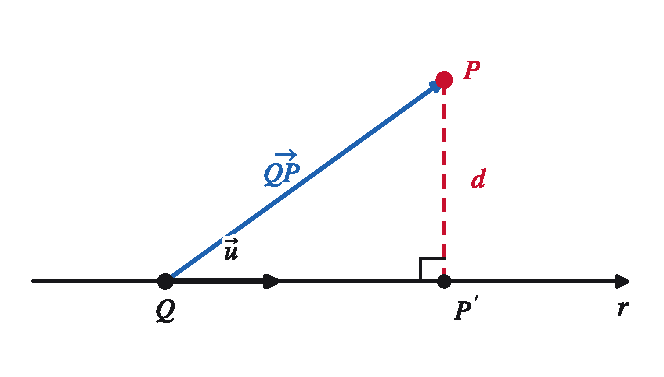
\includegraphics[width=319pt]{fig/m11_f22.pdf}
\caption{Distància del punt $P$ a la recta $r$: $d = |\vec u\times\overrightarrow{QP}|\,/\,|\vec u|$.}
\end{figure}

\section{Distància d'un punt a un pla}

La distància del punt $P(x_0, y_0, z_0)$ al pla $\pi: Ax + By + Cz + D = 0$ és $d(P, \pi) = d(P, P')$, on $P'$ és el peu de la perpendicular. La fórmula directa és:

\begin{equation*}
d(P, \pi) = \frac{|Ax_0 + By_0 + Cz_0 + D|}{\sqrt{A^2 + B^2 + C^2}}
\end{equation*}

\begin{figure}[!htbp]
\centering
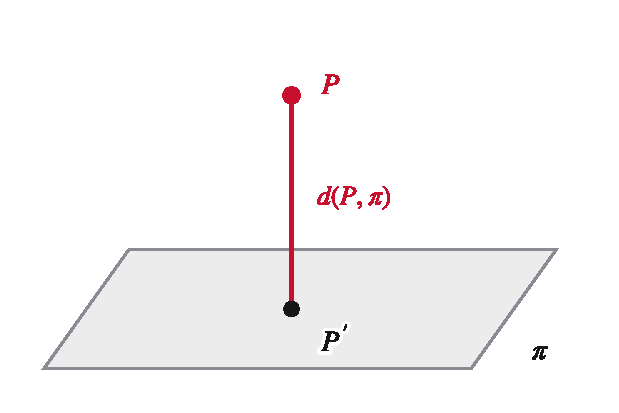
\includegraphics[width=297pt]{fig/m11_f23.pdf}
\caption{Distància del punt $P$ al pla $\pi$: la longitud del segment perpendicular a $\pi$ que passa per $P$.}
\end{figure}

\section{Distàncies entre rectes i plans}

\subsection{Distància entre dues rectes}

\begin{itemize}
\item \textbf{Secants o coincidents:} $d = 0$.
\item \textbf{Paral\textperiodcentered{}leles:} $d(r, s) = d(P, s)$, on $P$ és qualsevol punt de $r$.
\item \textbf{Que s'encreuen:} existeix una única recta $t$ perpendicular a ambdues. Si $P \in r$ i $P' \in s$ són els punts de contacte de $t$, aleshores $d(r, s) = d(P, P')$. Fórmula amb el producte mixt (apartat 8):
\end{itemize}

\begin{equation*}
d(r, s) = \frac{|[\overrightarrow{PQ}, \vec u, \vec v]|}{|\vec u\times\vec v|}
\end{equation*}

on $P \in r$, $Q \in s$, $\vec u$ i $\vec v$ són els vectors directors de $r$ i $s$.

\subsection{Distància entre una recta i un pla}

\begin{itemize}
\item Si la recta talla el pla o hi és continguda: $d = 0$.
\item Si la recta és paral\textperiodcentered{}lela al pla: $d(r, \pi) = d(P, \pi)$, on $P$ és qualsevol punt de $r$.
\end{itemize}

\subsection{Distància entre dos plans}

\begin{itemize}
\item Si es tallen o són coincidents: $d = 0$.
\item Si són paral\textperiodcentered{}lels: $d(\pi_1, \pi_2) = d(P, \pi_2)$, on $P$ és qualsevol punt de $\pi_1$.
\end{itemize}

\section{Angles formats per rectes i plans}

L'angle entre dos vectors $\vec v$ i $\vec w$ és:

\begin{equation*}
\vec v\cdot\vec w = |\vec v|\,|\vec w|\cos\alpha \;\Longrightarrow\; \alpha = \arccos\frac{\vec v\cdot\vec w}{|\vec v|\,|\vec w|}
\end{equation*}

\subsection{Angle entre dues rectes}

L'angle format per $r$ i $s$ és el més petit dels angles formats pels seus vectors directors $\vec u$ i $\vec v$ (es pren valor absolut per garantir un angle agut):

\begin{equation*}
\cos\alpha = \frac{|\vec u\cdot\vec v|}{|\vec u|\,|\vec v|} \;\Rightarrow\; \alpha = \arccos\frac{|\vec u\cdot\vec v|}{|\vec u|\,|\vec v|}
\end{equation*}

\subsection{Angle entre una recta i un pla}

L'angle $\alpha$ entre la recta $r$ (vector director $\vec u$) i el pla $\pi$ (vector normal $\vec n$) és el complement de l'angle $\beta$ entre $\vec u$ i $\vec n$:

\begin{equation*}
\sin\alpha = \cos\beta = \frac{|\vec u\cdot\vec n|}{|\vec u|\,|\vec n|} \;\Rightarrow\; \alpha = \arcsin\frac{|\vec u\cdot\vec n|}{|\vec u|\,|\vec n|}
\end{equation*}

\begin{figure}[!htbp]
\centering
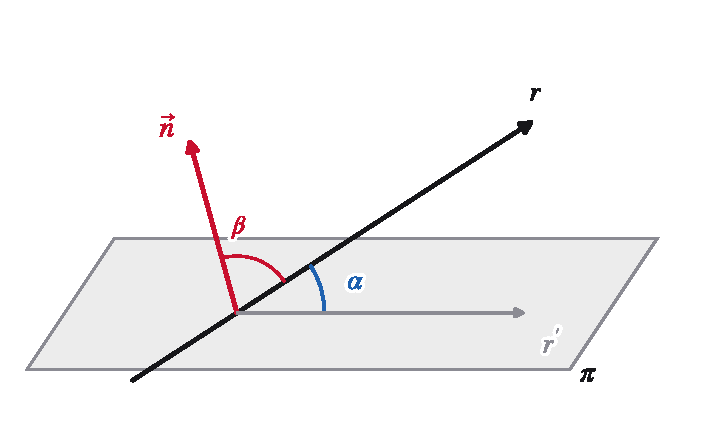
\includegraphics[width=341pt]{fig/m11_f24.pdf}
\caption{Angle $\alpha$ entre la recta $r$ i el pla $\pi$: $\sin\alpha = \cos\beta = |\vec u\cdot\vec n|\,/\,(|\vec u||\vec n|)$.}
\end{figure}

\subsection{Angle entre dos plans}

L'angle entre $\pi_1$ i $\pi_2$ (amb vectors normals $\vec n_1$ i $\vec n_2$) és el més petit dels angles diedres:

\begin{equation*}
\cos\alpha = \frac{|\vec n_1\cdot\vec n_2|}{|\vec n_1|\,|\vec n_2|} \;\Rightarrow\; \alpha = \arccos\frac{|\vec n_1\cdot\vec n_2|}{|\vec n_1|\,|\vec n_2|}
\end{equation*}

\section{Producte vectorial de dos vectors}

\textbf{Definició:} El \textbf{producte vectorial} de $\vec u = (u_1, u_2, u_3)$ i $\vec v = (v_1, v_2, v_3)$ és el vector

\begin{equation}
\vec u\times\vec v = \begin{vmatrix} \vec e_1 & u_1 & v_1 \\ \vec e_2 & u_2 & v_2 \\ \vec e_3 & u_3 & v_3 \end{vmatrix} = (u_2v_3 - u_3v_2,\; u_3v_1 - u_1v_3,\; u_1v_2 - u_2v_1)
\end{equation}

Les característiques del vector $\vec u\times\vec v$ són:

\begin{itemize}
\item \textbf{Mòdul:} $|\vec u\times\vec v| = |\vec u|\,|\vec v|\sin\alpha$, amb $0^\circ \le \alpha \le 180^\circ$.
\item \textbf{Direcció:} perpendicular als dos vectors $\vec u$ i $\vec v$.
\item \textbf{Sentit:} el d'avanç d'un tirabuixó que giri de $\vec u$ a $\vec v$ en el menor angle possible (regla de la mà dreta).
\end{itemize}

\emph{Observació:} si $\vec u\cdot\vec v = 0$, els vectors són perpendiculars i $|\vec u\times\vec v| = |\vec u|\,|\vec v|$ (valor màxim).

\section{Aplicacions geomètriques del producte vectorial}

\subsection{Àrea d'un paral\textperiodcentered{}lelogram}

Si $\vec u$ i $\vec v$ són dos costats adjacents del paral\textperiodcentered{}lelogram:

\begin{equation*}
A = |\vec u\times\vec v|
\end{equation*}

\subsection{Àrea d'un triangle}

Donats tres vèrtexs $P$, $Q$, $R$:

\begin{equation*}
A = \frac12\,|\overrightarrow{PQ}\times\overrightarrow{PR}|
\end{equation*}

\subsection{Distància d'un punt a una recta (forma alternativa)}

Si $Q \in r$ i $\vec u$ és el vector director de $r$:

\begin{equation*}
d(P, r) = \frac{|\vec u\times\overrightarrow{QP}|}{|\vec u|}
\end{equation*}

\section{Producte mixt de tres vectors}

\textbf{Definició:} El \textbf{producte mixt} dels vectors $\vec u$, $\vec v$ i $\vec w$ és el nombre real

\begin{equation}
[\vec u, \vec v, \vec w] = \vec u\cdot(\vec v\times\vec w) = \begin{vmatrix} u_1 & u_2 & u_3 \\ v_1 & v_2 & v_3 \\ w_1 & w_2 & w_3 \end{vmatrix}
\end{equation}

\section{Aplicacions geomètriques del producte mixt}

\subsection{Volum d'un paral\textperiodcentered{}lelepípede}

Si $\vec u$, $\vec v$ i $\vec w$ són tres arestes adjacents:

\begin{equation*}
V = |[\vec u, \vec v, \vec w]|
\end{equation*}

\subsection{Volum d'una piràmide de base triangular}

\begin{equation*}
V = \frac16\,|[\vec u, \vec v, \vec w]|
\end{equation*}

\subsection{Distància entre dues rectes que s'encreuen}

Si $P \in r$, $Q \in s$, i $\vec u$, $\vec v$ són els vectors directors de $r$ i $s$:

\begin{equation*}
|[\overrightarrow{PQ}, \vec u, \vec v]| = |\vec u\times\vec v|\cdot d(r, s) \;\Longrightarrow\; d(r, s) = \frac{|[\overrightarrow{PQ}, \vec u, \vec v]|}{|\vec u\times\vec v|}
\end{equation*}

\section{Complement: punts i figures simètriques}

\subsection{Mètode general}

El \textbf{simètric} $P'$ d'un punt $P$ respecte d'un element (punt, recta o pla) es troba trobant primer el \textbf{punt mitjà} $M$ entre $P$ i $P'$ i després aïllant:

\begin{equation*}
M=\frac{P+P'}{2}\quad\Longrightarrow\quad P'=2M-P
\end{equation*}

\begin{table}[!htbp]
\centering
\renewcommand{\arraystretch}{1.3}
\begin{tabularx}{\textwidth}{l>{\raggedright\arraybackslash}X}
\toprule
Respecte de\ldots{} & Com trobar $M$ \\
\midrule
un punt $Q$ & $M=Q$ \\
una recta $r$ & $M=r\cap\pi$, on $\pi$ és el pla per $P$ \textbf{perpendicular} a $r$ (vector normal $=\vec d_r$) \\
un pla $\pi$ & $M=r\cap\pi$, on $r$ és la recta per $P$ \textbf{perpendicular} a $\pi$ (vector director $=\vec n_\pi$) \\
\bottomrule
\end{tabularx}
\end{table}

\begin{figure}[!htbp]
\centering
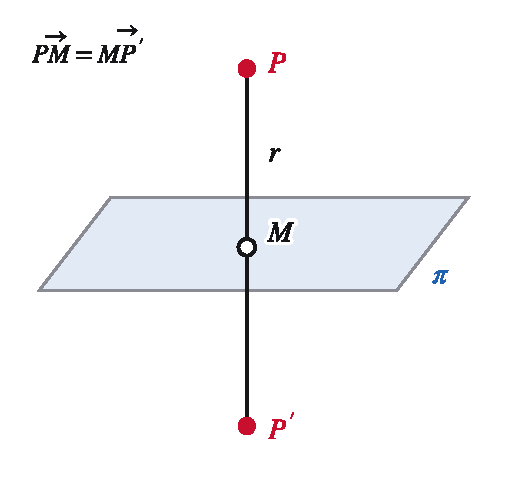
\includegraphics[width=251pt]{fig/m11_f37.pdf}
\caption{El simètric $P'$ de $P$ respecte d'un pla: $M$ és la intersecció de la perpendicular $r$ amb el pla i és el punt mitjà de $PP'$.}
\end{figure}

\subsection{Exemple 1 --- Simètric respecte d'un pla}

Simètric de $P(1,2,3)$ respecte de $\pi:\ x+y+z-3=0$.

\begin{enumerate}
\item Recta perpendicular per $P$: $r:\ (1+t,\,2+t,\,3+t)$.
\item Intersecció amb $\pi$: $(1+t)+(2+t)+(3+t)-3=0\Rightarrow 3+3t=0\Rightarrow t=-1$, de manera que $M=(0,1,2)$.
\item $P'=2M-P=(2\cdot0-1,\,2\cdot1-2,\,2\cdot2-3)=(-1,0,1)$.
\end{enumerate}

\emph{Comprovació:} $-1+0+1-3=-3$ i $1+2+3-3=3$: estan a banda i banda del pla i a la mateixa distància $\checkmark$.

\subsection{Exemple 2 --- Simètric respecte d'una recta}

Simètric de $P(1,2,0)$ respecte de $r:\ (t,\,t,\,0)$ amb $\vec d=(1,1,0)$.

\begin{enumerate}
\item Pla per $P$ perpendicular a $r$: $x+y+D=0$ i $1+2+D=0\Rightarrow D=-3$, així que $\pi:\ x+y-3=0$.
\item $M=r\cap\pi$: $t+t-3=0\Rightarrow t=\frac32$ i $M=\left(\frac32,\frac32,0\right)$.
\item $P'=2M-P=(3-1,\,3-2,\,0)=(2,1,0)$.
\end{enumerate}

\subsection{Pla mediador}

El \textbf{pla mediador} d'un segment $AB$ és el pla perpendicular a $AB$ pel seu punt mitjà: conté tots els punts equidistants d'$A$ i $B$.

\emph{Exemple:} $A(1,0,2)$ i $B(3,2,0)$. $\overrightarrow{AB}=(2,2,-2)\parallel(1,1,-1)$ i $M=(2,1,1)$. Llavors $x+y-z+D=0$ amb $2+1-1+D=0\Rightarrow D=-2$:

\begin{equation*}
\pi:\ x+y-z-2=0
\end{equation*}

\section{Complement: interpretació geomètrica dels productes vectorial i mixt}

\begin{figure}[!htbp]
\centering
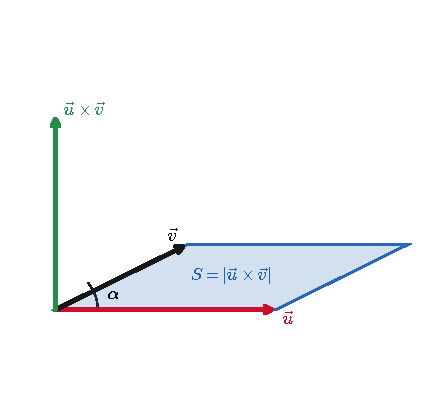
\includegraphics[width=208pt]{fig/x11_cross.pdf}
\caption{El producte vectorial $\vec u\times\vec v$ és perpendicular al pla que formen $\vec u$ i $\vec v$ (regla de la mà dreta) i el seu mòdul és l'àrea del paral\textperiodcentered{}lelogram.}
\end{figure}

El sentit de $\vec u\times\vec v$ es determina amb la \textbf{regla de la mà dreta}: si els dits van de $\vec u$ cap a $\vec v$ pel camí més curt, el polze indica el sentit del producte. Per això $\vec v\times\vec u=-\,\vec u\times\vec v$.

\begin{figure}[!htbp]
\centering
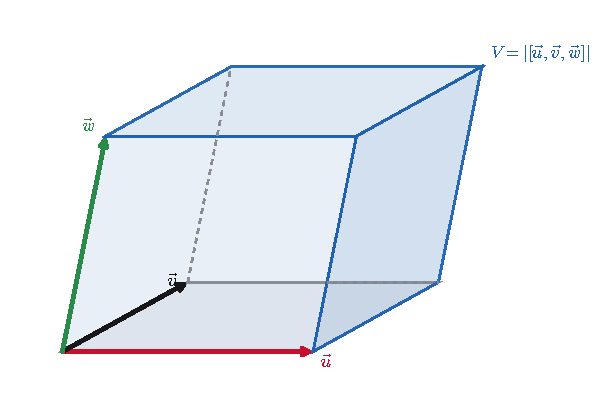
\includegraphics[width=286pt]{fig/x11_parallelepiped.pdf}
\caption{El valor absolut del producte mixt $[\vec u,\vec v,\vec w]$ és el volum del paral\textperiodcentered{}lelepípede definit pels tres vectors.}
\end{figure}

El producte mixt es calcula com a determinant: $[\vec u,\vec v,\vec w]=\begin{vmatrix}u_1&u_2&u_3\\v_1&v_2&v_3\\w_1&w_2&w_3\end{vmatrix}$. Si val $0$, els tres vectors són coplanaris.

\section{Complement: exemples resolts de distàncies, angles i volums}

\emph{Exemple 1 --- Distància d'un punt a un pla:} $P(1,2,3)$ i $\pi:\ 2x-y+2z-4=0$:

\begin{equation*}
d(P,\pi)=\frac{|2\cdot1-2+2\cdot3-4|}{\sqrt{2^2+(-1)^2+2^2}}=\frac{2}{3}.
\end{equation*}

\emph{Exemple 2 --- Distància entre dues rectes que s'encreuen:} $r:(0,0,0)+t(1,0,0)$ i $s:(0,1,0)+u(0,0,1)$. $\vec u\times\vec v=(0,-1,0)$, $\overrightarrow{PQ}=(0,1,0)$ i $[\vec u,\vec v,\overrightarrow{PQ}]=-1$:

\begin{equation*}
d(r,s)=\frac{|[\vec u,\vec v,\overrightarrow{PQ}]|}{|\vec u\times\vec v|}=\frac11=1.
\end{equation*}

\emph{Exemple 3 --- Angle entre dos plans:} $\pi:x+y+z=0$ i $\pi':x+y=0$, amb $\vec n=(1,1,1)$ i $\vec n'=(1,1,0)$:

\begin{equation*}
\cos\alpha=\frac{|\vec n\cdot\vec n'|}{|\vec n|\,|\vec n'|}=\frac{2}{\sqrt3\,\sqrt2}=\frac{2}{\sqrt6}\ \Rightarrow\ \alpha\approx35{,}3^{\circ}.
\end{equation*}

\emph{Exemple 4 --- Angle entre una recta i un pla:} $r$ de vector director $\vec u=(1,2,2)$ i el pla $z=0$ ($\vec n=(0,0,1)$): $\sin\alpha=\dfrac{|\vec u\cdot\vec n|}{|\vec u|\,|\vec n|}=\dfrac23\Rightarrow\alpha\approx41{,}8^{\circ}$.

\emph{Exemple 5 --- Àrea d'un triangle i volum d'un tetraedre:} Siguin $A(1,0,0)$, $B(0,2,0)$, $C(0,0,3)$ i $O(0,0,0)$.

\begin{itemize}
\item $\overrightarrow{AB}=(-1,2,0)$ i $\overrightarrow{AC}=(-1,0,3)$; $\overrightarrow{AB}\times\overrightarrow{AC}=(6,3,2)$ amb mòdul $7$. Àrea del triangle $ABC=\dfrac72$.
\item El volum del tetraedre $OABC$ és $\dfrac16\bigl|[\overrightarrow{OA},\overrightarrow{OB},\overrightarrow{OC}]\bigr|=\dfrac16\cdot6=1$.
\item El pla $ABC$ és $\dfrac x1+\dfrac y2+\dfrac z3=1$, és a dir, $6x+3y+2z-6=0$, i la distància d'$O$ a aquest pla és $\dfrac{6}{7}$. Comprovació: $V=\dfrac13\cdot\dfrac72\cdot\dfrac67=1$.
\end{itemize}

\emph{Exemple 6 --- Distància d'un punt a una recta:} $P(1,1,1)$ i $r:(0,0,0)+t(1,0,0)$. $\overrightarrow{QP}=(1,1,1)$ i $\vec u\times\overrightarrow{QP}=(0,-1,1)$, de mòdul $\sqrt2$: $d(P,r)=\dfrac{\sqrt2}{1}=\sqrt2$.
